\chapter{Implementation}
This chapter will present the implementation phase of the thesis project and explain the main concepts in the implementation.\\

The literature rewiev provided good insight in the subject of lane detection systems and paved the way for starting the implementation phase of the project. However, one important issue was brought up  regarding the image acquisition on the Zynq-7000 board due to lack of camera drivers. A decision to use a separate node for the image processing part was made and is described more in detail in this section.
\section{EMC2 board specification}
The mixed criticality platform that Alten uses can either be a Zedboard or an $EMC^2$-board. Both these boards hardware consists of a Xilinx Zynq-7000 which consists of an dual-core ARM-Cortex-A9 processor as well as an programmable logic part (FPGA). 
\section{Raspberry pi}
This section will describe the single board computer that is used for lane detection in this degree project. The chosen board is a Raspberry Pi 3 which is a credit card sized computer. The third generation of the raspberry has seen some major hardware updates compared to earlier versions. The one used in this project has the following specifications:


\begin{table}[H]
\centering
\caption{Raspberry Pi 3 Model B specifications}
\label{my-label}
\begin{tabular}{lllll}
 Model:	&Raspberry Pi 3 Model B  \\
 Operating system:	&Rasbian-Jessie  \\
 Processor:	&ARM Cortex-A53 1.2 GHz 64-bit quad-core  \\
 Hardware Ports:	&40 GPIO pins, 4 USB ports, HDMI port, Ethernet port,\\  &3.5 mm audio jack, Camera interface, Display interface,\\  &Micro SD card slot
\end{tabular}
\end{table}


The main computer in this project is the Zynq-7000 board and thus it would be preferred to utilize it for the lane detection as well. But due to no camera drivers available for the Zynq-7000 board it would be difficult to manage the image acquisition. A search for other hardware that is more suitable for the task was carried out and the raspberry pi was chosen due to that it is widely used in computer vision projects and its affordable price point.

\begin{figure}[H]
  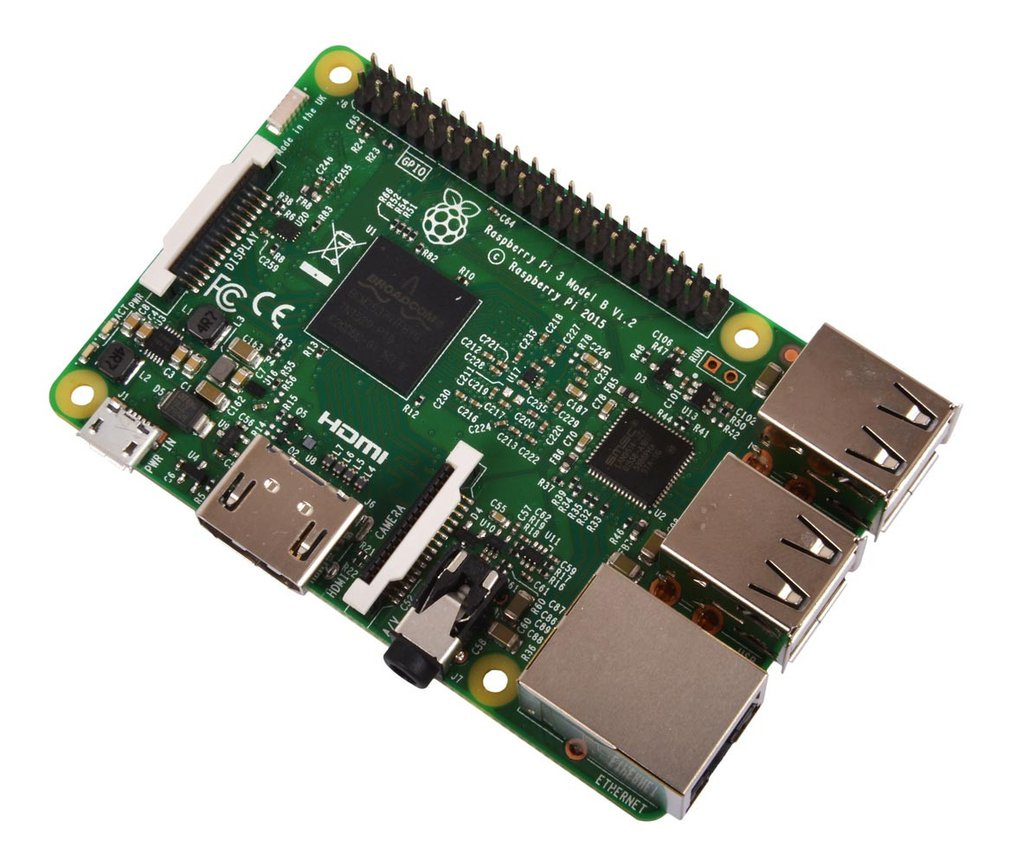
\includegraphics[scale=0.3]{./img/rpi.jpg}
  \centering
  \caption{Raspberry Pi 3}
  \label{fig:RPI}
\end{figure}

\subsection{Pi camera}
The Raspberry Pi camera module has been chosen as image acquisition device for this project. The camera module has a five megapixel image sensor and a maximum resolution of 2952 x 1944 pixels. This camera was chosen due the fact that it is made specifically for the raspberry pi and is very easy to use. The one used has a very wide angle lens which turned out to entail both advantages and disadvantages. The positive thing with a wide angle lens is the wide image that the camera can capture so it can see the road in almost all angles. The negative thing with the wide angle lens is that the image is quite distorted at the edges, which makes the angle calculations less accurate. 



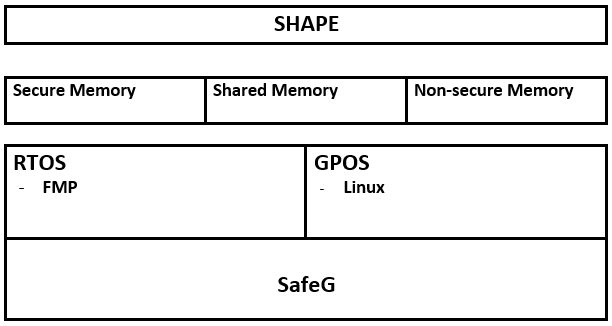
\includepdf[scale=0.8,pages=1,pagecommand=\section{System architecture}]{./img/architecture.pdf}


\section{System identification}
To know how the system will behave when being fed with different PWM values an experimental setup has been developed and many (136) different PWM inputs and steering angle outputs have been measured.


\begin{figure}[H]
  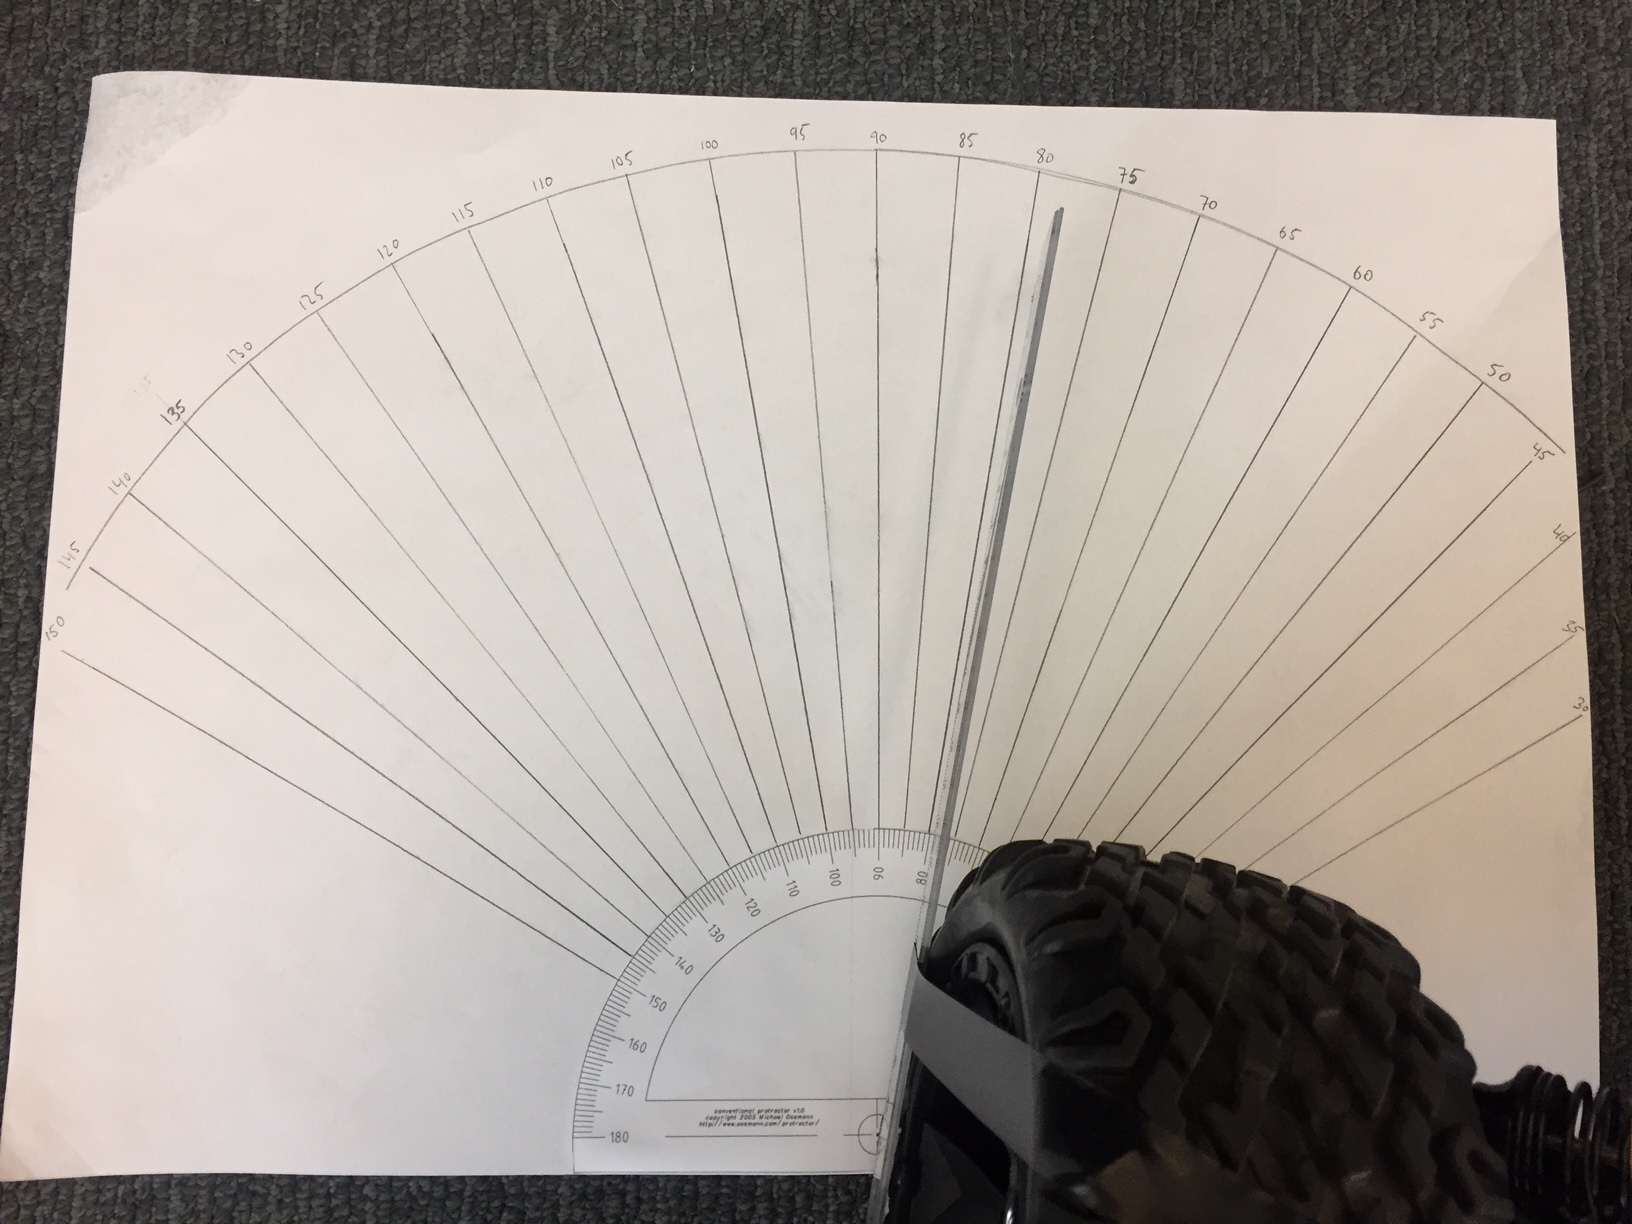
\includegraphics[width=\textwidth]{./img/anglepic.JPG}
  \centering
  \caption{Angle measurement}
  \label{fig:Angle measurement}
\end{figure}


The mean value of the angle outputs have been calculated and and a first order polynomial have been fitted to the data points using the least squares method. The line calculated is shown in figure  \ref{fig:PWM and angle correlation} and has the equation $$ y=-14.26x + 195.96$$ 

\begin{figure}[H]
  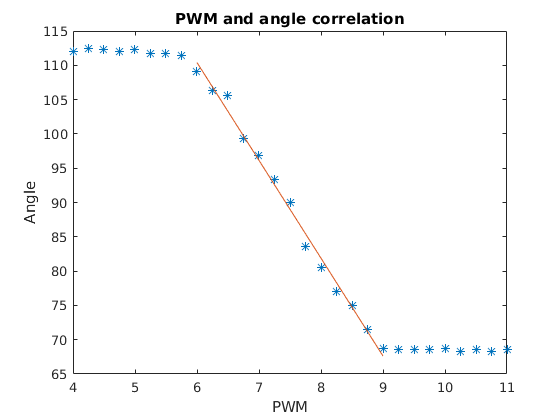
\includegraphics[width=\textwidth]{./img/PWMPLOT_2.png}
  \centering
  \caption{PWM and angle correlation}
  \label{fig:PWM and angle correlation}
\end{figure}

The angles in figure \ref{fig:PWM and angle correlation} are defined as in table \ref{Steering angle and direction} below.

\begin{table}[H]
\centering
\caption{Steering angle and direction}
\label{Steering angle and direction}
\begin{tabular}{@{} cl @{}}
\toprule
Angle		& Direction \\ 
\midrule
 \textless 90		& Left turn \\ 
  \: 90		& Straight forward \\ 
 \textgreater 90		& Right turn \\ 
\bottomrule
 \end{tabular}
\end{table}


The line equation calculated is used in the steering control system to evaluate the steering angle compared to the identified line angles. This process is described later in this chapter.\\

This is used in combination with the position control to eliminate the deviation from the centerline and thus improve performance of the system.


\section{Lane detection algorithm}
This chapter will describe the algorithms used for lane detection that have been implemented on the demonstrator of this project.\\

The algorithm that has been implemented on the demonstrator so far consist of the following steps:\\

The lane detection process starts with grabbing a frame from the Raspberry Pi camera and applying a few preprocessing steps to the image.\\

The first step is to crop the image to only contain the region of interest (ROI). This is a camera setting that can be predefined so that the camera only grabs the ROI and thus not need to crop it after the frame is grabbed.\\

The following step is to convert the image to gray scale to prepare it for next coming operations. Figure \ref{fig:Input image and grayscale} below shows how the acquired image looks in the first stages of the lane detection process.

\begin{figure}[H]
  \begin{subfigure}[b]{0.50\textwidth}
    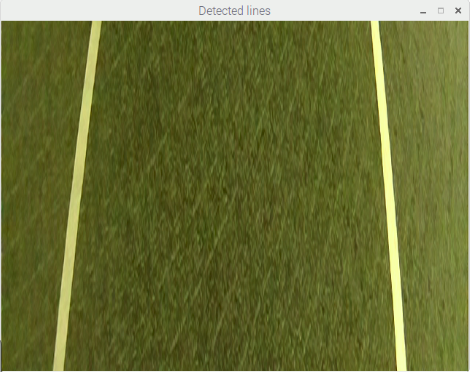
\includegraphics[width=\textwidth]{./img/input22.png}
    \caption{\label{fig:input image}Input image}
  \end{subfigure}
  \begin{subfigure}[b]{0.50\textwidth}
    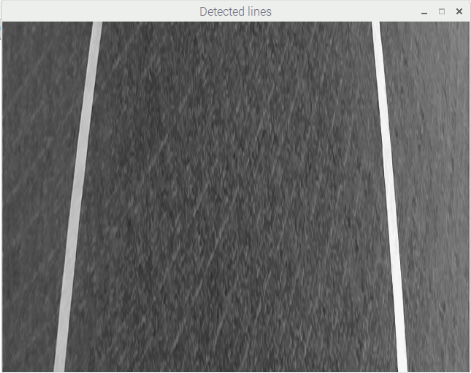
\includegraphics[width=\textwidth]{./img/gray22.png}
    \caption{\label{fig:gray image}Converted to grayscale}
  \end{subfigure}
  \caption{\label{fig:Input image and grayscale}Input image before and after grayscale filter}
\end{figure}


The gray scale image is the input to the canny edge detection function. As described in the state of the art section the output of the canny function is a thresholded image where all the pixels that are part of edges are set to white and all pixels that are not part of edges are set black. Using the OpenCV library function Canny, figure \\ref{fig:Input image and grayscale} is obtained.

\begin{figure}[H]
  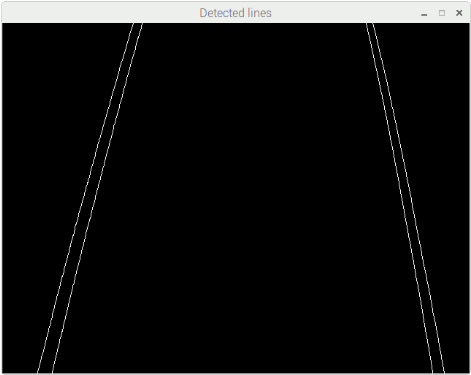
\includegraphics[width=\textwidth]{./img/edges22.png}
  \centering
  \caption{Tresholded image using canny filter}
  \label{fig:Tresholded image using canny filter}
\end{figure}

This thresholded image is used as an input to the Hough transform function that is used for line detection.


\begin{figure}[H]
  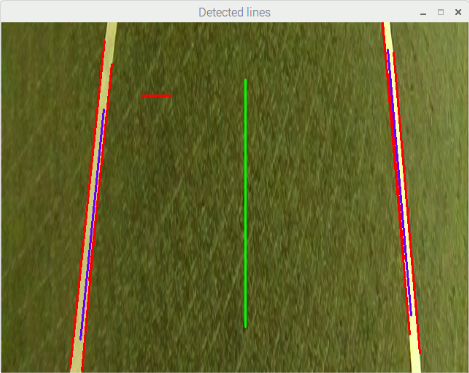
\includegraphics[width=\textwidth]{./img/detected.png}
  \centering
  \caption{Detected lines}
  \label{fig:Detected lines}
\end{figure}

The were a lot of problems when developing the algorithm in terms of false positives when evaluating the lines in the image. A solution was developed in order to eliminate the false lines in the image and only keep the the lines that are part of a road lane.\\

The concept behind this lane detection algorithm solution is to group lines in the image that are very close to each other. So for instance if we find several lines on both the left and right lane of the road, these form two groups of lines because the lines are close to each other. If there are other lines in the image that are not very close to these two lanes, they will be put in separate groups. There can be multiple groups depending on how many false lines that are detected. In the end the groups are evaluated and the two groups with the most number of lines in them are the one that are regarded as lanes. The short red horizontal line visible in \ref{fig:Detected lines} is the threshold distance for lines to be grouped in the same group.\\

This gives a very robust lane detection algorithm that disregards false positives from the hough transform.\\

What happens if a new line is introduced in the image that is not part of the road lanes?

\begin{figure}[H]
  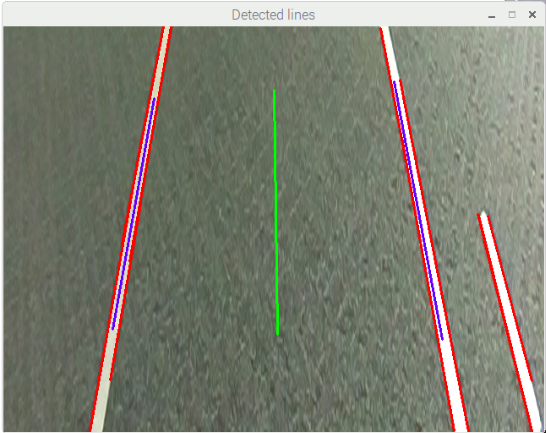
\includegraphics[width=\textwidth]{./img/falsepositive.png}
  \centering
  \caption{False positive line}
  \label{fig:angle}
\end{figure}

In the image above one extra line has been introduced and is detected by the system. But due to the concept of grouping lines and evaluating which ones are the most prominent, it is clear in this case that the system disregards from the new line and indicates the center and direction of the road correctly. 



\section{Lateral control}
Now the lines are detected and the vehicle need to be controled in some way using the information from the lane detection. So far all of these steps are all done on the Raspberry Pi thanks to its easy camera implementation and that it supports OpenCV.\\

There are two errors that are calculated and from which the vehicle is controlled by. The positional error is calculated by splitting the image into two halves and making the assumption that we have one lane in each of the two halves. A centerline is calculated from the two lanes and by measuring the distance from the centerline to the middle of the image, the error is calculated as $$error_{pos} = x\_mid\_camera - x\_mid\_center\_lane$$

The other error used for control is the angle by which the vehicle is travelling forward compared to the angle of the road. This is calculated from the captured images and compared to the vehicles angle with the information from the system identification.\\

\begin{figure}[H]
  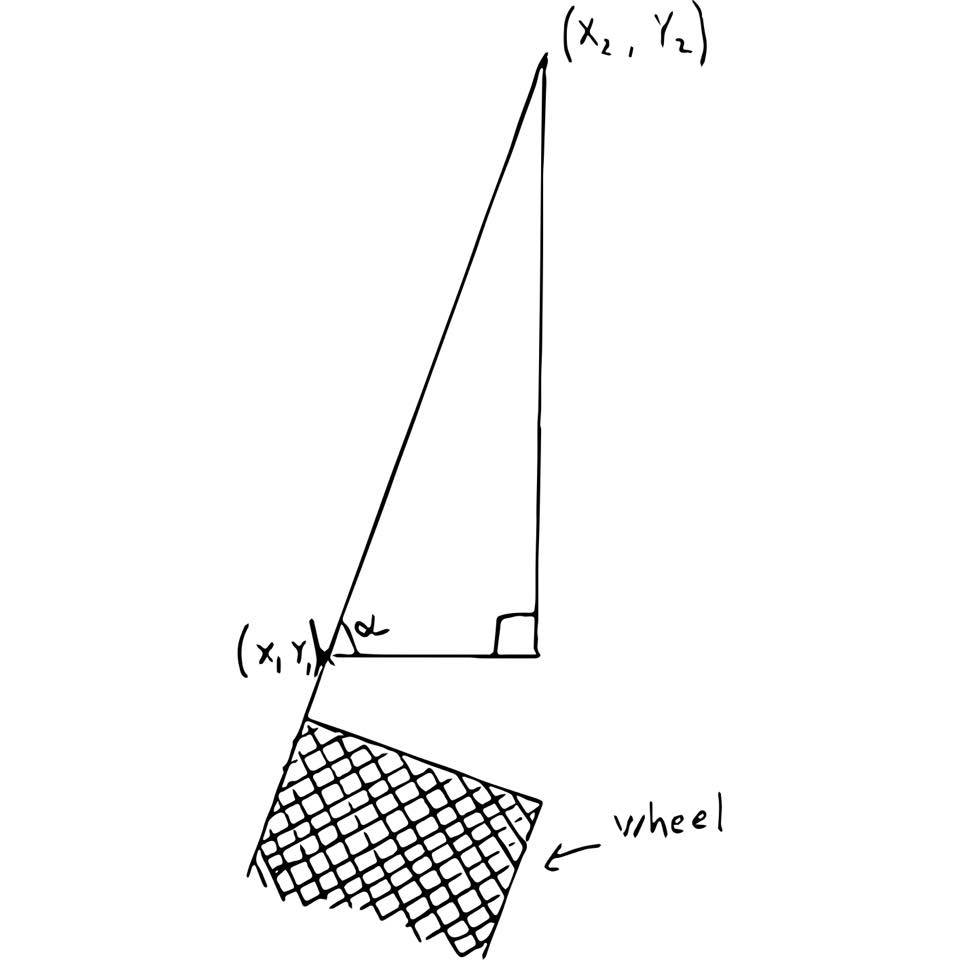
\includegraphics[scale=0.25]{./img/angle.JPG}
  \centering
  \caption{Angle calculation}
  \label{fig:angle}
\end{figure}


In the captured images from the camera the angle of the centerline can be calculated using the known x and y values. The x in the picture is calculated as $$x = abs(x1-x2)$$ and y is calculated as $$y=abs(y1-y2)$$ and the angle is obtained using $$tan(\alpha)=\frac{y}{x}$$ and thus $$\alpha = arctan(\frac{y}{x})$$

This $\alpha$ angle is compared to the known angle from the system identification and an $error_{angle}$ is calculated

$$error_{angle} = \alpha - (u*(-14.26)+195.96)$$


The two errors are sent to the EMC2 board via serial communication where the lateral control is scheduled and executed on the mixed criticality platform.\\

A PID controller for the steering servo is developed using z transform. The output signal u to the steering servo is calculated as:
$$u = \frac{PWM_{min}+PWM_{max}}{2} - a_{angle}*error_{angle} + a_{pos}*error_{pos}$$

\section{Implementation and integration with zedboard}
\subsection{Tasks}
As shown in figure \ref{fig:sequence diagram} there are currently threeXXX tasks scheduled that run on the real time operating system.

\begin{figure}[H]
  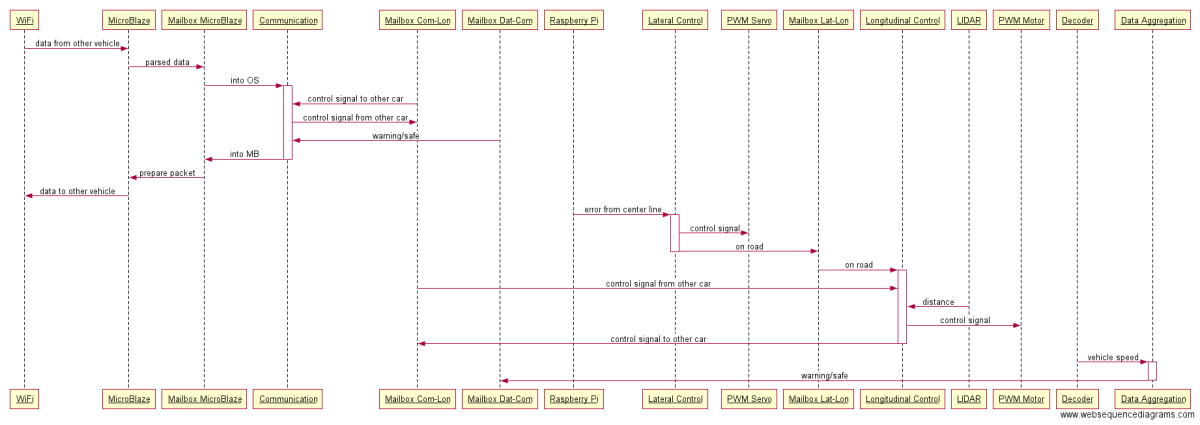
\includegraphics[width=\textwidth]{./img/sekvensdiagram.png}
  \centering
  \caption{Sequence diagram}
  \label{fig:sequence diagram}
\end{figure}
The tasks implemented on the board are described below.
 
\subsubsection{Communication}
In this task all the vehicle-to-vehicle (V2V) communication and vehicle-to-infrastructure (V2I) communication is done. The information that is sent is

\begin{itemize}
  \item Current state of vehicle
  \item Current speed of vehicle
  \item Distance to vehicle in front
  \item Longitudinal control signal
  \item Lateral control signal
\end{itemize}

\subsubsection{Lateral control}
In this task the lateral control described earlier is executed.
\subsubsection{Data aggregation}
The data aggregation task is combining sensor data in order to detect anomalies, which could mean slippage of one wheel or other information which can useful to share to other vehicles within the ITS.  
\subsubsection{Longitudinal control}
This task controls the distance to the vehicle in front of the platoon. The distance is measured using the LIDAR.\\
 
There will eventually be more tasks implemented including one task to switch to the non-critical operating system.

\subsection{Priority}
All the tasks are scheduled with fixed priority. The prority of the tasks are:

\begin{enumerate}
  \item Communication
  \item Lateral control
  \item Data aggregation
  \item Longitudinal control
\end{enumerate}


\subsection{Timing requirements}
WCET for the lateral control task is calculated as the end-to-end time which starts from the image acquisition in the Raspberry Pi, to the control signal that the emc2 sends. 